\documentclass[]{article}
\usepackage{lmodern}
\usepackage{amssymb,amsmath}
\usepackage{ifxetex,ifluatex}
\usepackage{fixltx2e} % provides \textsubscript
\ifnum 0\ifxetex 1\fi\ifluatex 1\fi=0 % if pdftex
  \usepackage[T1]{fontenc}
  \usepackage[utf8]{inputenc}
\else % if luatex or xelatex
  \ifxetex
    \usepackage{mathspec}
  \else
    \usepackage{fontspec}
  \fi
  \defaultfontfeatures{Ligatures=TeX,Scale=MatchLowercase}
\fi
% use upquote if available, for straight quotes in verbatim environments
\IfFileExists{upquote.sty}{\usepackage{upquote}}{}
% use microtype if available
\IfFileExists{microtype.sty}{%
\usepackage{microtype}
\UseMicrotypeSet[protrusion]{basicmath} % disable protrusion for tt fonts
}{}
\usepackage[margin=1in]{geometry}
\usepackage{hyperref}
\hypersetup{unicode=true,
            pdftitle={Statistical Machine Learning: Midterm},
            pdfauthor={Oussama Azizi A07922203},
            pdfborder={0 0 0},
            breaklinks=true}
\urlstyle{same}  % don't use monospace font for urls
\usepackage{graphicx,grffile}
\makeatletter
\def\maxwidth{\ifdim\Gin@nat@width>\linewidth\linewidth\else\Gin@nat@width\fi}
\def\maxheight{\ifdim\Gin@nat@height>\textheight\textheight\else\Gin@nat@height\fi}
\makeatother
% Scale images if necessary, so that they will not overflow the page
% margins by default, and it is still possible to overwrite the defaults
% using explicit options in \includegraphics[width, height, ...]{}
\setkeys{Gin}{width=\maxwidth,height=\maxheight,keepaspectratio}
\IfFileExists{parskip.sty}{%
\usepackage{parskip}
}{% else
\setlength{\parindent}{0pt}
\setlength{\parskip}{6pt plus 2pt minus 1pt}
}
\setlength{\emergencystretch}{3em}  % prevent overfull lines
\providecommand{\tightlist}{%
  \setlength{\itemsep}{0pt}\setlength{\parskip}{0pt}}
\setcounter{secnumdepth}{0}
% Redefines (sub)paragraphs to behave more like sections
\ifx\paragraph\undefined\else
\let\oldparagraph\paragraph
\renewcommand{\paragraph}[1]{\oldparagraph{#1}\mbox{}}
\fi
\ifx\subparagraph\undefined\else
\let\oldsubparagraph\subparagraph
\renewcommand{\subparagraph}[1]{\oldsubparagraph{#1}\mbox{}}
\fi

%%% Use protect on footnotes to avoid problems with footnotes in titles
\let\rmarkdownfootnote\footnote%
\def\footnote{\protect\rmarkdownfootnote}

%%% Change title format to be more compact
\usepackage{titling}

% Create subtitle command for use in maketitle
\newcommand{\subtitle}[1]{
  \posttitle{
    \begin{center}\large#1\end{center}
    }
}

\setlength{\droptitle}{-2em}

  \title{Statistical Machine Learning: Midterm}
    \pretitle{\vspace{\droptitle}\centering\huge}
  \posttitle{\par}
    \author{Oussama Azizi A07922203}
    \preauthor{\centering\large\emph}
  \postauthor{\par}
    \date{}
    \predate{}\postdate{}
  
\textbackslash{}documentclass{[}fontset=ubuntu,UTF8,a4paper,
11pt{]}\{ctexart\}
\usepackage{ctex}
\usepackage[utf8x]{inputenc}

\begin{document}
\maketitle

\section{1. Exploratory Data Analysis}\label{exploratory-data-analysis}

We look at the summary of the data :

\begin{verbatim}
##      Income           Limit           Rating          Cards      
##  Min.   : 10.35   Min.   :  855   Min.   : 93.0   Min.   :1.000  
##  1st Qu.: 21.01   1st Qu.: 3088   1st Qu.:247.2   1st Qu.:2.000  
##  Median : 33.12   Median : 4622   Median :344.0   Median :3.000  
##  Mean   : 45.22   Mean   : 4736   Mean   :354.9   Mean   :2.958  
##  3rd Qu.: 57.47   3rd Qu.: 5873   3rd Qu.:437.2   3rd Qu.:4.000  
##  Max.   :186.63   Max.   :13913   Max.   :982.0   Max.   :9.000  
##       Age          Education        Gender    Student   Married  
##  Min.   :23.00   Min.   : 5.00   Female:207   No :360   No :155  
##  1st Qu.:41.75   1st Qu.:11.00   Male  :193   Yes: 40   Yes:245  
##  Median :56.00   Median :14.00                                   
##  Mean   :55.67   Mean   :13.45                                   
##  3rd Qu.:70.00   3rd Qu.:16.00                                   
##  Max.   :98.00   Max.   :20.00                                   
##             Ethnicity      Balance       
##  African American: 99   Min.   :   0.00  
##  Asian           :102   1st Qu.:  68.75  
##  Caucasian       :199   Median : 459.50  
##                         Mean   : 520.01  
##                         3rd Qu.: 863.00  
##                         Max.   :1999.00
\end{verbatim}

We notice that the classes are imbalanced : Indeed, \(50\%\) of
participants are Caucasians, and only \(25\%\) are African American and
\(25\%\) Asian. To address this issue, we perform the Synthetic Minority
Over-sampling Technique (SMOTE) and we obtain the following result :

\begin{verbatim}
## African American            Asian        Caucasian 
##              297              133              263
\end{verbatim}

Hence we have \(42.85\%\) proportion of African American \(20.63\%\) of
Asian and \(36.50\%\) of Caucasian which is more balanced than the
previous proportions. Using \(Ggobi\) we visualize the multivariate
parallel plot to check if there are some outliers :

\begin{figure}
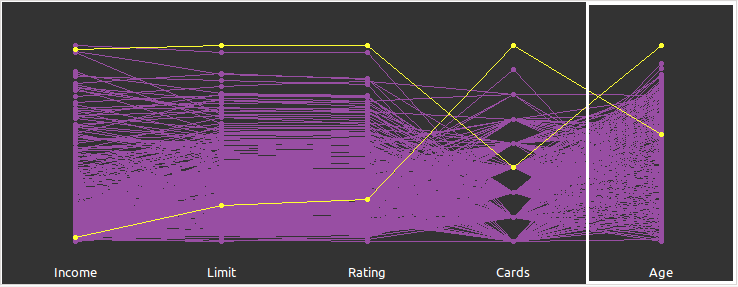
\includegraphics[width=1\linewidth]{plots/potential outliers 384 & 324} \caption{A caption}\label{fig:pressure}
\end{figure}

We notice that the observation \(324\) and \(384\) are potential
outliers, we hence delete them from the dataset. We use the
z-standardization to normalize the data for algorithms that are
sensitive to scaling such as SVM for which features with higher variance
have larger effect on the margin. We plot boxplots for each explanatory
variable:

\begin{center}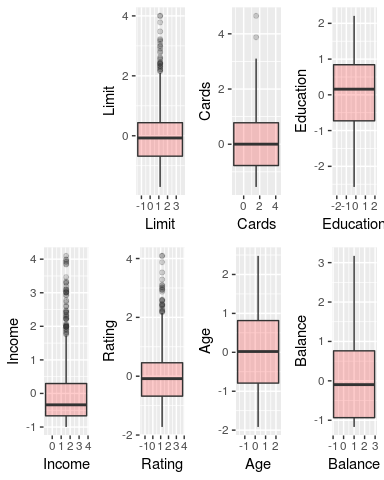
\includegraphics{Report_files/figure-latex/unnamed-chunk-3-1} \end{center}

We conclude that there are few leverage points but we won't drop them
since they don't affect that much the results compared to outliers. We
plot the histograms for each explanatory variable for each class :

\begin{center}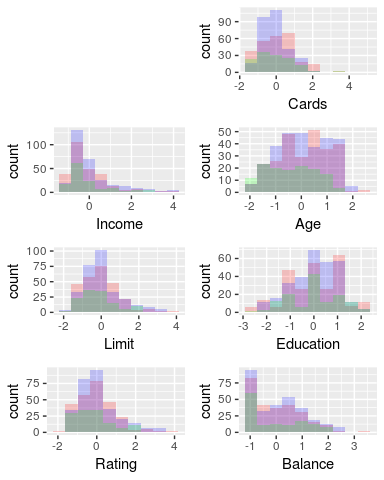
\includegraphics{Report_files/figure-latex/unnamed-chunk-4-1} \end{center}

The first observation that we notice is that all the classes overlap for
every explanatory variable, which might be an indicator of bad
explanatory variables selection. This will make the classification
process difficult to achieve and will lead to very poor performance as
we will see. To confirm this, we use the T-distributed Stochastic
Neighbor Embedding (T-SNE) to visualize the data in 2 dimensions:

\begin{center}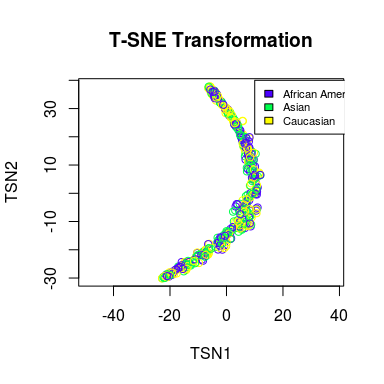
\includegraphics{Report_files/figure-latex/unnamed-chunk-5-1} \end{center}

The second observation is that the distribution of features for each
class are either right skewed or left skewed which violates the
multivariate normality assumption, since joint normality implies
marginal one.

\section{2. Single Learners}\label{single-learners}

For each single classifier,we use 10-fold Cross-validation to estimate
the true error and we use the latter as a metric to compare between
these models. The ROC would have been a good metric if we didn't solve
the problem of imbalanced classes and if we had only two classes.

\subsection{2.1 LDA and QDA}\label{lda-and-qda}

\subsubsection{Checking LDA and QDA
assumptions}\label{checking-lda-and-qda-assumptions}

LDA and QDA requires that the predictors are normally distributed for
each class. As we have seen from the histograms of features, the
distributions are either left or right skewed but not normal. We perform
a Mardia's test to make sure that it is the case :

\begin{verbatim}
##              Test        Statistic               p value Result
## 1 Mardia Skewness 875.299004709567 5.43999099243476e-132     NO
## 2 Mardia Kurtosis 3.01542845755448   0.00256616470035986     NO
## 3             MVN             <NA>                  <NA>     NO
\end{verbatim}

As we see, the predictors marginal distribution didn't pass the Mardia's
test for kurtosis nor the skewness one for normality. Another condition
is that the covariance matrix should be the same for the outcome across
all class groups.

\begin{center}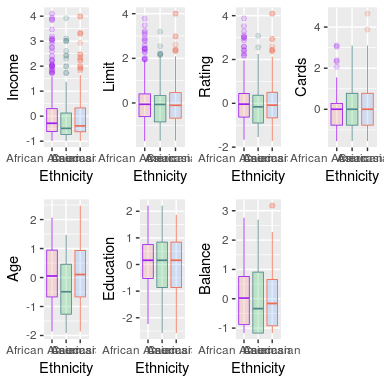
\includegraphics{Report_files/figure-latex/unnamed-chunk-7-1} \end{center}

Except for Education, All the other predictors have different
Covariances accross the space groups. To assess this issue, we are going
to run a Box's M test, even if it is sensible when multivariate
normality is not verified:

\begin{verbatim}
## 
##  Box's M-test for Homogeneity of Covariance Matrices
## 
## data:  credit2[features]
## Chi-Sq (approx.) = 184.77, df = 56, p-value = 1.148e-15
\end{verbatim}

We can clearly see that the \(p-value << 0.05\) which indicates high
evidence against the null hypothesis
\(H_0 : The \space covariance \space matrices \space of \space the \space Ethnicity \space variable \space are \space equal \space across \space all \space groups \space .\)
We can also perform a Levene's test which is more relevant since the
data is not normal:

\begin{verbatim}
## [1] "Cards~Ethnicity"
\end{verbatim}

\begin{verbatim}
## Levene's Test for Homogeneity of Variance (center = median)
##        Df F value    Pr(>F)    
## group   2  14.216 8.908e-07 ***
##       690                      
## ---
## Signif. codes:  0 '***' 0.001 '**' 0.01 '*' 0.05 '.' 0.1 ' ' 1
\end{verbatim}

\begin{verbatim}
## [1] "Balance~Ethnicity"
\end{verbatim}

\begin{verbatim}
## Levene's Test for Homogeneity of Variance (center = median)
##        Df F value Pr(>F)
## group   2  1.7891 0.1679
##       690
\end{verbatim}

\begin{verbatim}
## [1] "Age~Ethnicity"
\end{verbatim}

\begin{verbatim}
## Levene's Test for Homogeneity of Variance (center = median)
##        Df F value Pr(>F)
## group   2  0.1243 0.8832
##       690
\end{verbatim}

\begin{verbatim}
## [1] "Rating~Ethnicity"
\end{verbatim}

\begin{verbatim}
## Levene's Test for Homogeneity of Variance (center = median)
##        Df F value Pr(>F)
## group   2   0.294 0.7454
##       690
\end{verbatim}

We conclude that apart from the variable \(Cards\) the covariances seem
to be homogenious. Again the homogeneous covariance assumption is
violated. We should expect the LDA to perform bad and QDA better since
it is not affected by the variance-covariance heterogeneity. We perform
10-fold Cross validation to estimate the true error of both LDA and QDA.
We plot the confusion matrix for both classifiers :

\begin{center}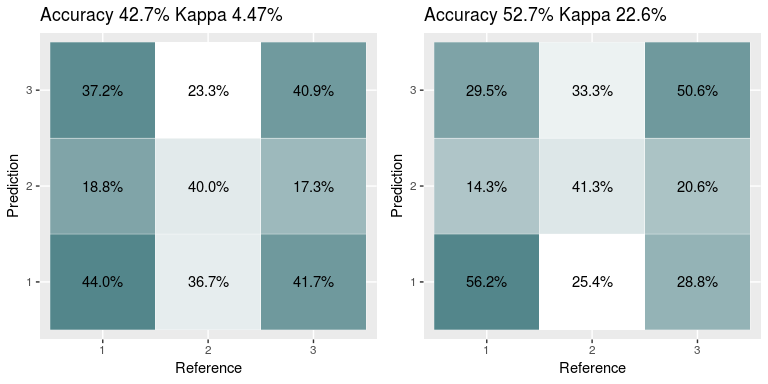
\includegraphics{Report_files/figure-latex/unnamed-chunk-10-1} \end{center}

On the left, the confusion matrix of LDA indicates an estimate true
error of \(43.1\%\) while the confusion matrix of QDA indicates an
estimate true error of \(51.1\%\).

\subsection{2.2 Support Vector Machine}\label{support-vector-machine}

We use the default settings for kernel for SVM, and a 10-fold cross
validation to find the best values for the parameter \(\gamma\) and the
cost \(c\). To serve this purpose, we make a grid search for the best
\((c,\gamma)\) in the space \([0.1,15] \times [0.5,5]\).

\begin{center}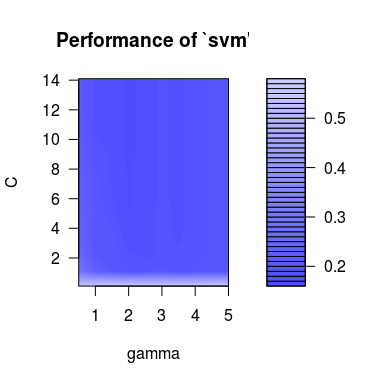
\includegraphics{Report_files/figure-latex/unnamed-chunk-11-1} \end{center}

The best value of the pair \((c,\gamma)\) is \((6.1,2)\) which leads to
an apparent error of \(15.15\%\). We test the model on the test set. We
obtain the confusion matrix resulting of the 10-fold cross validation :

\begin{center}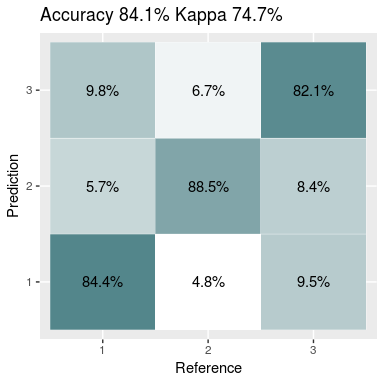
\includegraphics{Report_files/figure-latex/unnamed-chunk-12-1} \end{center}

According to the 10-fold Cross-validation the true error is estimated to
\(15.9\%\).

\subsection{2.3 Decision Tree}\label{decision-tree}

For this part we will develop a decision tree model based on the
previous features. For this purpose we split the data into training set
and test set and we use the \(rpart\) function of \(rpart\) library,
which builds a decision tree using the training set and estimates the
missclassification error using 10-fold Cross-validation. We obtain the
following Error versus Tree size graph:

\begin{center}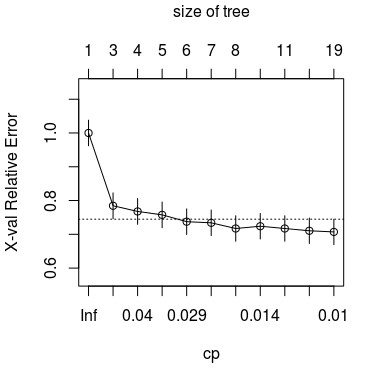
\includegraphics{Report_files/figure-latex/unnamed-chunk-13-1} \end{center}

We noticed that the missclassification error never goes down below
\(0.1\), hence the 1-SE rule cannot be applied to choose the ideal tree
size. We will also note that, even with 10 fold-cross validation we do
not obtain consistent missclassifcation errors as we run the code
several times. This can be explained by the fact that decision trees are
unstable to very small variations especially that the distribution of
predictors overlap. It would have hence be better if we had a larger
dataset or other predictors. However this issue can be solved using
Ensemble methods. The maximum tree size gives us an accuracy of
\(56.3218391\%\). We use postpruning to have a compromise between tree
size and missclassification error with a complexity parameter of
\(cp = 0.011 \space\) which gives us a very large tree :

\begin{center}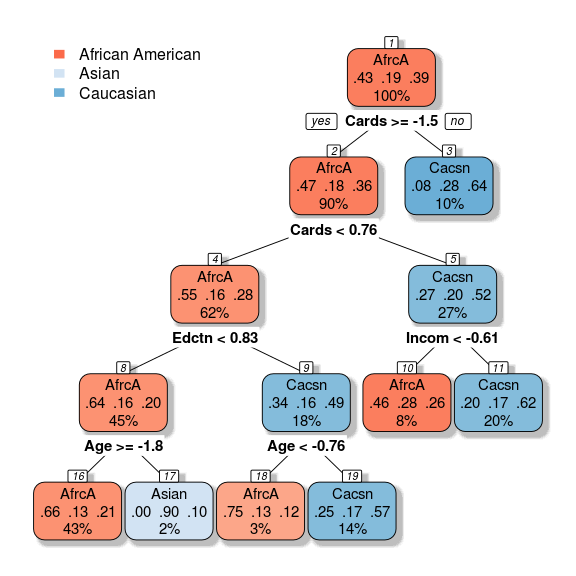
\includegraphics{Report_files/figure-latex/unnamed-chunk-14-1} \end{center}

The accuracy of the pruned tree is \(50\%\).

\subsection{2.4 Logistic discrimination}\label{logistic-discrimination}

In this part, we construct a multinomial logistic classifier using the
\(multinom\) function of the \(nnet\) package. We construct the model
using a training set from the total data set.

By looking at the deviance we should expect a low accuracy on the test
set. The confusion matrix for the test set is as following:

\begin{center}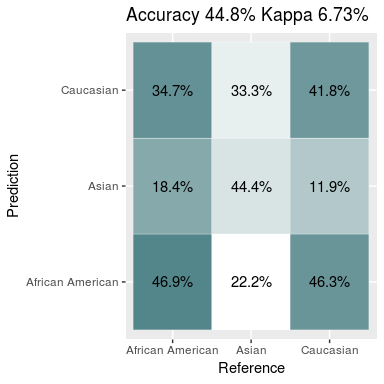
\includegraphics{Report_files/figure-latex/unnamed-chunk-16-1} \end{center}

The Multinomial logistic classifier performs as poorly as the LDA
classifier with an accuracy of \(44.8275862\%\).

\subsection{2.5 KNN}\label{knn}

We perform a K-Nearest Neighbors algorithm using the \(caret\) package.
We split once again the data to training set and a test set and we
perform a 10-fold Cross Validation using the training to obtain the best
value of \(K\).

\begin{center}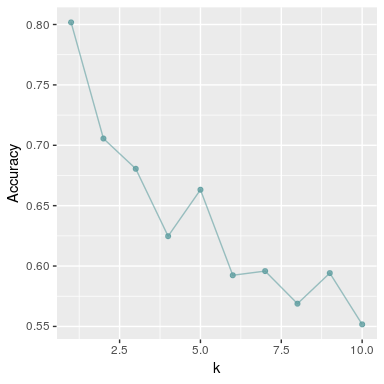
\includegraphics{Report_files/figure-latex/unnamed-chunk-17-1} \end{center}

It seems that the best value is \(K=1\) with a accuracy of
\(80.1752526\%\). We make predictions on the test test and we obtain the
following confusion matrix:

\begin{center}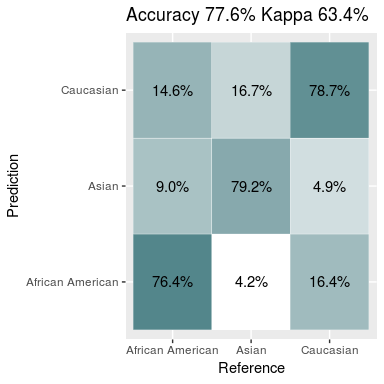
\includegraphics{Report_files/figure-latex/unnamed-chunk-18-1} \end{center}

Our model have a good accuracy on the test set : \(77.5862069\%\), but
still doesn't outperform SVM.

\subsection{2.6 Conclusion}\label{conclusion}

In this first part, we have seen \(6\) different classifiers and used
the missclassification error as a metric to assess their performance. To
conclude we can say that SVM has been the most effective algorithm and
LDA and the logistic classifier the less effective ones. We predict the
\(Ethnicity\) of participants in the data in the \(Test.txt\) file ,
using the obtained SVM algorithm. First of all, we normalize data using
the the z-standardization with the sample means and standard errors for
each feature of the first dataset, since the number of observations in
the \(Test.txt\) file is much lower than the total number of
observations of the first dataset. Using the SVM model that we created
earlier we obtain the following predictions:

\begin{table}

\caption{\label{tab:unnamed-chunk-19}A Knitr table.}
\centering
\begin{tabular}[t]{r|r|r|r|r|r|l|l|l|r|l}
\hline
Income & Limit & Rating & Cards & Age & Education & Gender & Student & Married & Balance & Ethnicity\\
\hline
14.312 & 5380 & 367 & 1 & 60 & 17 & Male & No & No & 1420 & Asian\\
\hline
98.515 & 8780 & 633 & 5 & 80 & 11 & Female & No & Yes & 1130 & African American\\
\hline
44.205 & 5641 & 414 & 2 & 32 & 12 & Female & No & Yes & 607 & African American\\
\hline
26.427 & 7533 & 433 & 5 & 50 & 15 & Male & Yes & Yes & 1304 & Caucasian\\
\hline
30.550 & 5869 & 439 & 7 & 83 & 8 & Female & No & No & 867 & Caucasian\\
\hline
\end{tabular}
\end{table}

\section{3. Ensemble methods}\label{ensemble-methods}

\subsection{3.1 Random Forest}\label{random-forest}

We perform a random forest using a number trees to grow of
\(m=2 \approx \sqrt{7}\) since we use \(7\) explanatory variables. We
obtain the following confusion matrix :

\begin{center}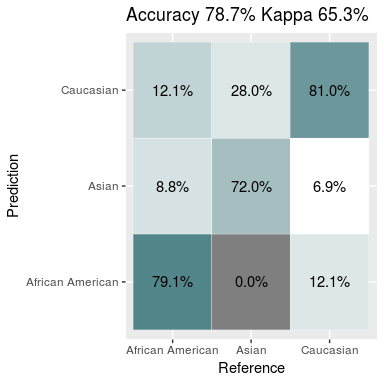
\includegraphics{Report_files/figure-latex/unnamed-chunk-20-1} \end{center}

We can see that performing a Random Forest has a huge impact on the
decision tree it doubles it's accuracy.

\subsection{3.2 Gradient boosting}\label{gradient-boosting}

We make a model of gradient boosting using a total number of trees of
\(5000\) and an interaction depth of \(6\), this results in the
following confusion matrix:

\begin{center}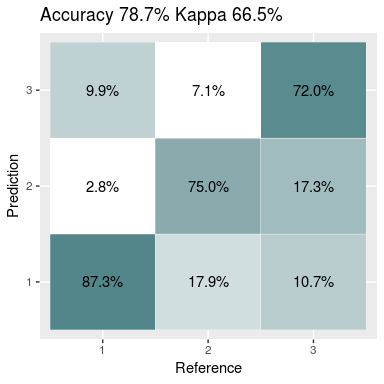
\includegraphics{Report_files/figure-latex/unnamed-chunk-21-1} \end{center}

Surprisingly the Gradient boosting model performs worse than the Random
Forest.

\section{4. Adding more explanatory
variables}\label{adding-more-explanatory-variables}

In this section we introduce the remaining categorical variables
\(Gender \space\), \(Student \space\) and \(Married \space\) and we use
decision rules to make the classification. Since these categorical
variables are binary, we don't need to add new dummy variables to the
data.

\section{4.1 Naïve Bayes}\label{naive-bayes}

We perform a 10-fold cross validation in order to estimate the true
accuracy of the Naive Bayes classifier

\begin{center}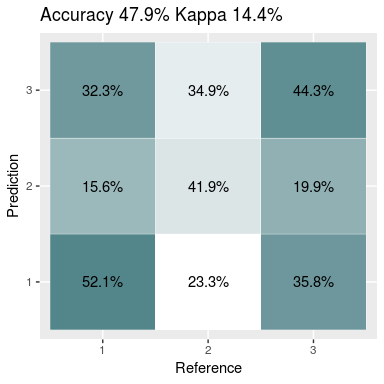
\includegraphics{Report_files/figure-latex/unnamed-chunk-22-1} \end{center}

The accuracy of the Naive Bayes classifier is very low as we can see.
This is probably due to the fact that the features are not independent.
A typical violation of this independence assumption is the possible
correlation between predictors, we can imagine that being a student is
correlated with being younger and having a lower income, and being
married correlated with being older and having a higher income since
married people tend to be older, hence they tend to be more experienced
in their jobs.

\section{4.2 Decision Tree}\label{decision-tree-1}

The second decision rule model that we use is the Decision Tree model.
We obtain the following Error versus Tree size for the traning set:

\begin{center}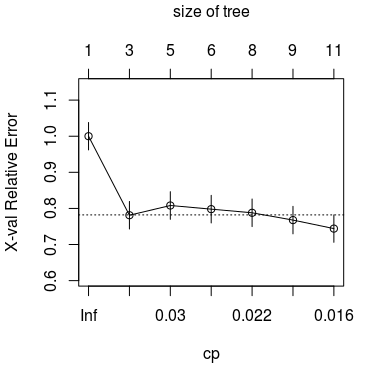
\includegraphics{Report_files/figure-latex/unnamed-chunk-23-1} \end{center}

We choose the complexity parameter \(cp = 0.014\) and we obtain the
following confusion matrix for the test set:

\begin{center}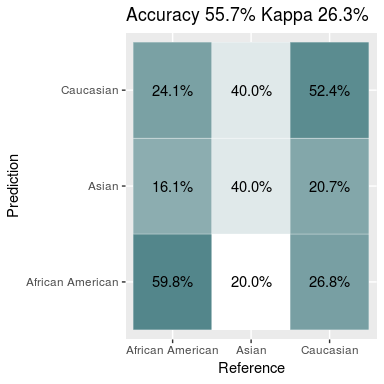
\includegraphics{Report_files/figure-latex/unnamed-chunk-24-1} \end{center}

The Decision Tree gained about \(5\%\) in Accuracy by adding the
categorical features and performes better than the Naive Bayes
Classifier. We are going to choose it to predict the Ethnicity of
participants in the \(Text.txt\) file. We obtain the following
predictions :

\begin{table}

\caption{\label{tab:unnamed-chunk-25}A Knitr table.}
\centering
\begin{tabular}[t]{r|r|r|r|r|r|l|l|l|r|l}
\hline
Income & Limit & Rating & Cards & Age & Education & Gender & Student & Married & Balance & Ethnicity\\
\hline
14.312 & 5380 & 367 & 1 & 60 & 17 & Male & No & No & 1420 & Asian\\
\hline
98.515 & 8780 & 633 & 5 & 80 & 11 & Female & No & Yes & 1130 & African American\\
\hline
44.205 & 5641 & 414 & 2 & 32 & 12 & Female & No & Yes & 607 & African American\\
\hline
26.427 & 7533 & 433 & 5 & 50 & 15 & Male & Yes & Yes & 1304 & Caucasian\\
\hline
30.550 & 5869 & 439 & 7 & 83 & 8 & Female & No & No & 867 & Caucasian\\
\hline
\end{tabular}
\end{table}

\section{5 Conclusion:}\label{conclusion-1}

In this project we performed a classification on a categorical data
using multiple approaches. The SVM model seems to be the best candidate
for this problem followed with KNN and Random Forest respectively.


\end{document}
